\section{Description of OpenVAS Setup} \label{sec:setup}

Open Vulnerability Assessment System is a system that collects multiple services and tools, called “Network Vulnerability Tests” (NVT) and presents them in a single interface, allowing the user to combine them to a thoroughly vulnerability scan \cite{openvas}. \\

\noindent The logical layout of the network scanned for this report is presented in Figure \ref{fig:setup}, where the target is “rome.secnet”. OpenVAS is installed on the intermediate server between the target and our client machine. \\

\noindent Scanning a host is a method to control in which ways a system is open to the outside, and it is one of the methods an attacker might conduct to search for entry points in a system \cite{wiki}. There are several types of vulnerability scans, such as “port scan”, “database scan”, “web application security scan” and others \cite{hk}. \\

\noindent The scans used in this report is in order: “port scan”, “service fingerprinting” and “network vulnerability scan”. The different scans will produce a list of open ports found on the host, combined with a fingerprint scan that will search through these open ports and generate a fingerprint of what type of services that are behind these ports. The fingerprint will contain the available information, such as the names and versions of services. \\

\noindent In the scans we expect a result in the form of information about open ports and the services behind them, marked with the security risk of each port and/or service.\\

\noindent To perform a scan with OpenVAS, the system needs to be installed on a server. In the interface of OpenVAS, the user choose which types of NVTs should be conducted with each scan, what port range to use and which target in the network the scan is aimed at. \\

\noindent To detect as many open ports as possible within a reasonable time, the optimized OpenVAS default port range was chosen. This setting checks a 
wide range of well known ports, and is optimized to lower the time 
consumption of the scan, compared to a scan over all ports.\\

%\noindent The aim of this report is to detect as many open ports as possible, within reason. The host is not known to have any extraordinary security issues, so the OpenVAS default port range was chosen as a suitable range, as it provides a wide range of well known ports.



\begin{figure}[hbt]
  \centering
  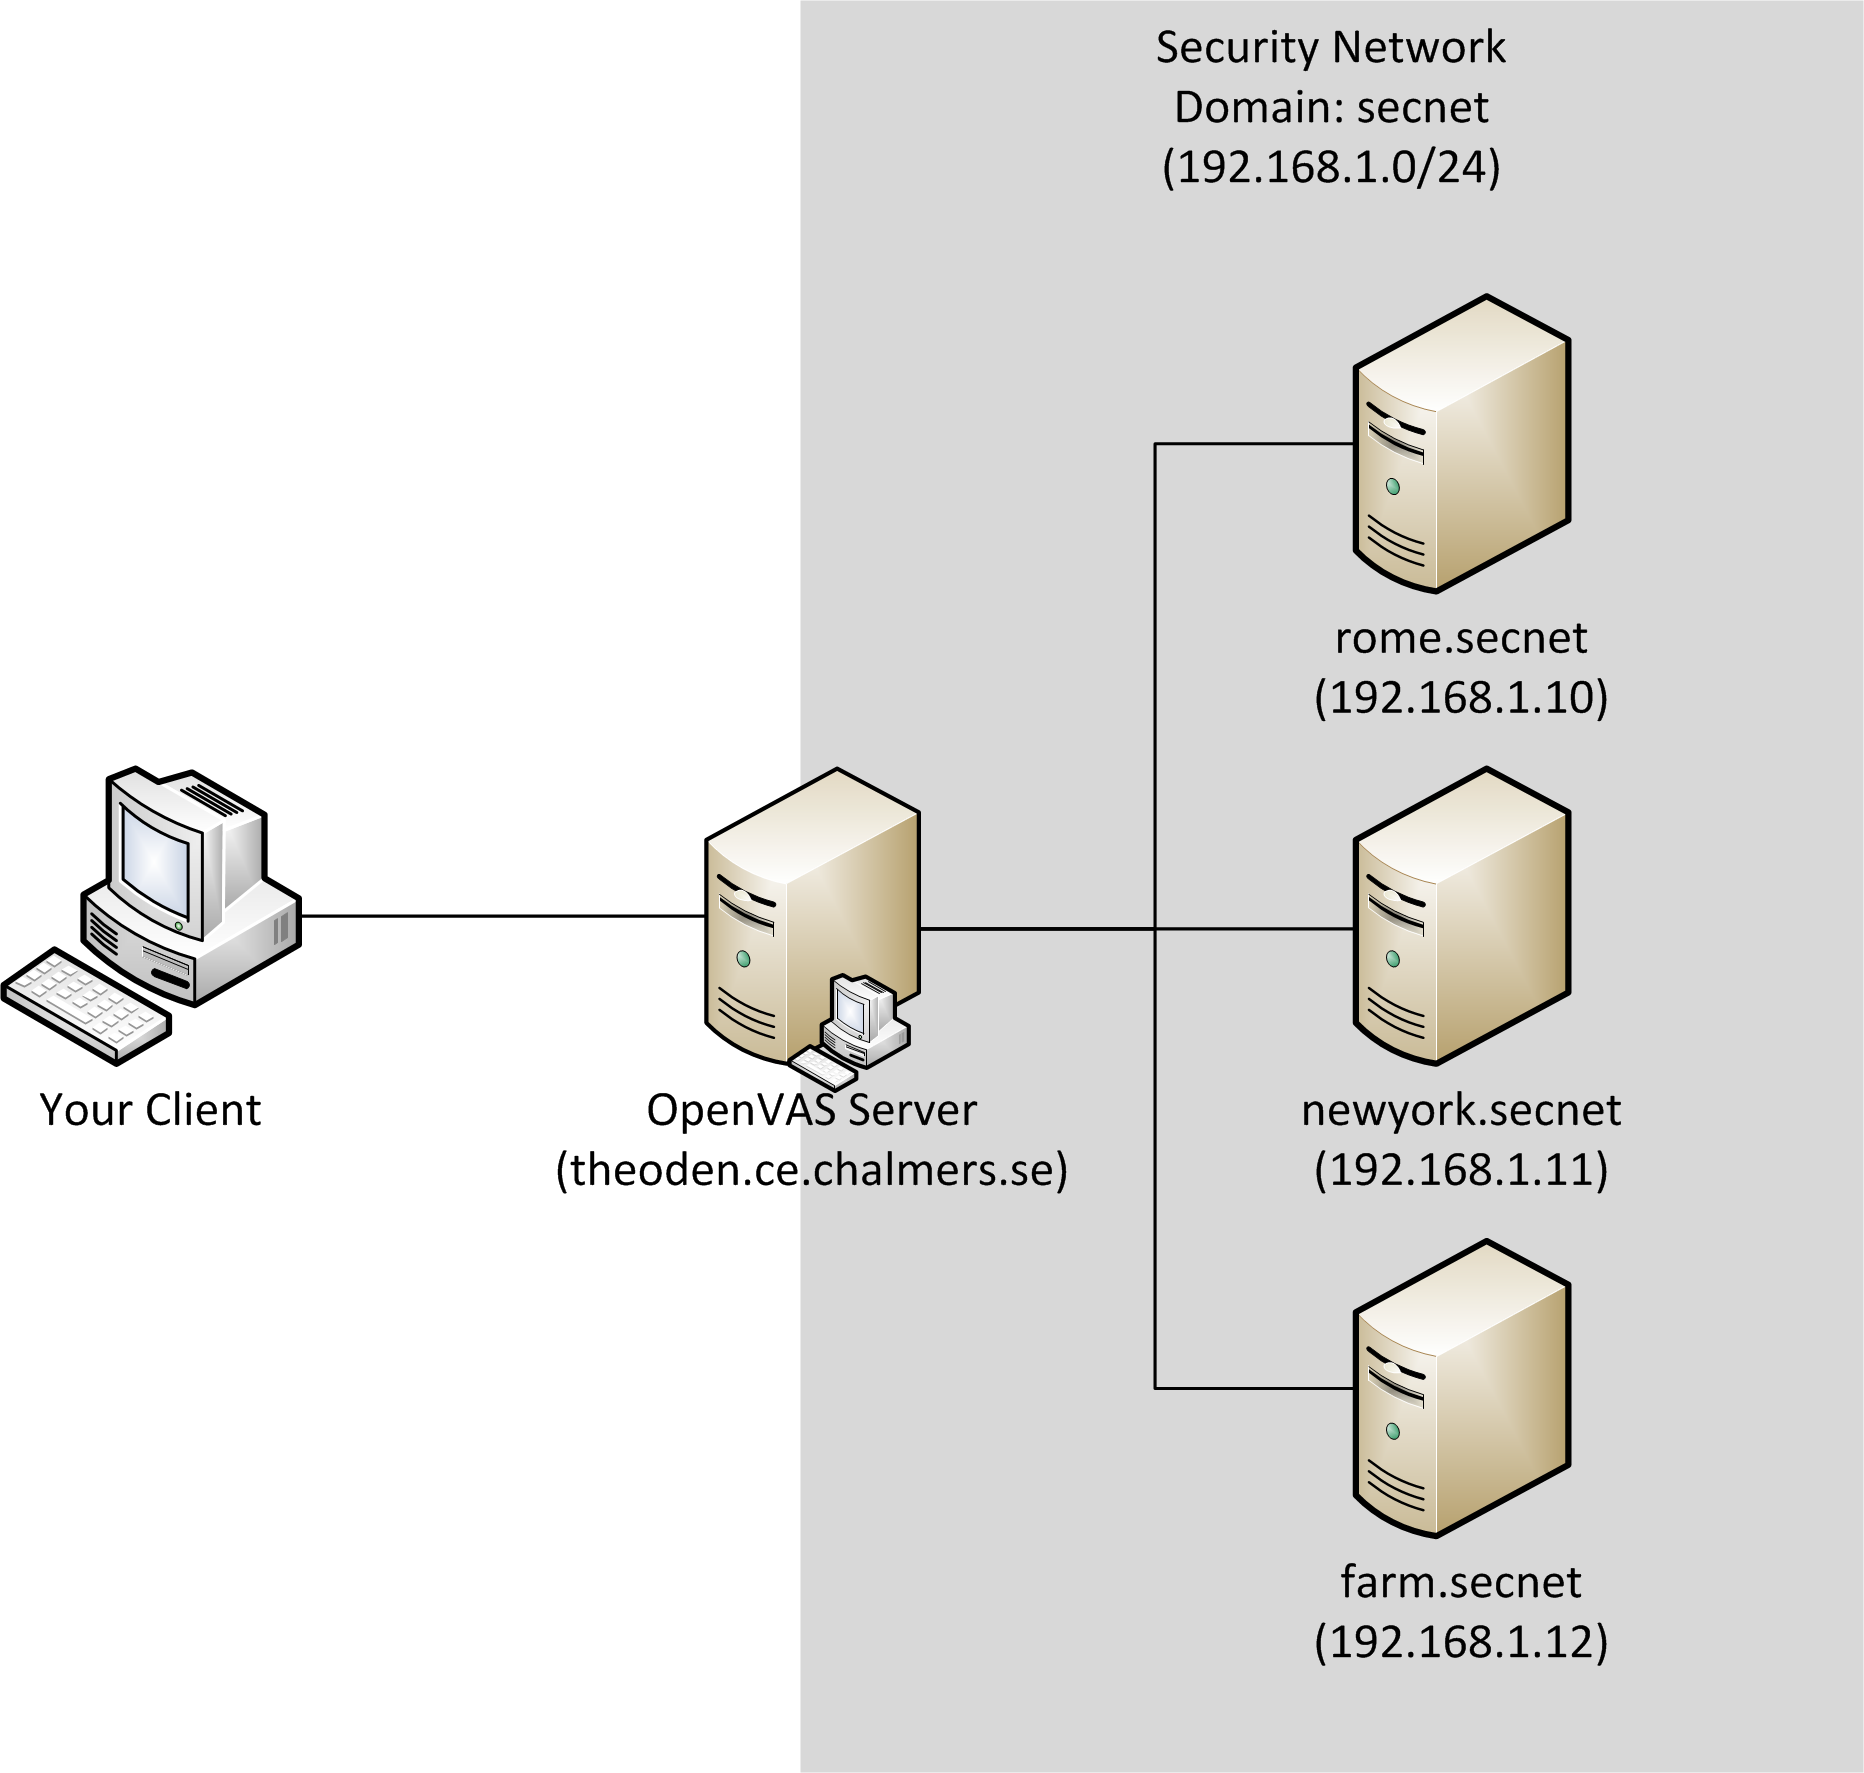
\includegraphics[scale=.4]{figures/setup.png}
  \caption{The network setup} \label{fig:setup}
\end{figure}



\subsection{Port Scanning}
\label{sub:port_set}

A set of tests in OpenVAS, called “Port Scanners”, were used to perform the port scanning, see Figure \ref{fig:portscanners}. \\

\noindent These NVTs where chosen so that a thorough port scan were conducted, and the open ports on the target will be displayed clearly. By doing this, information is gained on which ports on the target there are services listening for incoming connections. This is also similar to what a potential attacker would do.

\begin{figure}[htb]
  \centering
  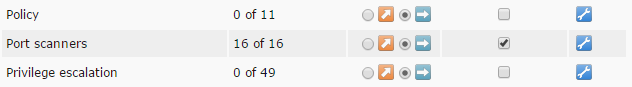
\includegraphics[scale=.4]{figures/port_nvt}
  \caption{Port Scanners NVT} \label{fig:portscanners}
\end{figure}

\newpage

\subsection{Service fingerprinting}
\label{sub:finger_set}
The settings we used in this section is the ones presented in Figures \ref{fig:general} and \ref{fig:service}

\begin{figure}[b!]
  \centering
  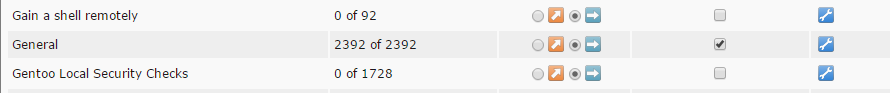
\includegraphics[scale=.4]{figures/general_nvt}
  \caption{General NVT} \label{fig:general}
\end{figure}

\begin{figure}[b!]
  \centering
  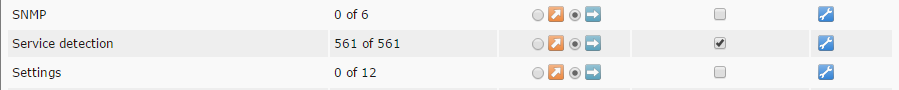
\includegraphics[scale=.4]{figures/service_nvt}
  \caption{Service detection NVT} \label{fig:service}
\end{figure}

\subsubsection{Service Fingerprinting}
To see which kind of services are running on the target system, OpenVAS was set up to try to get identifying information from them. Here the NVT families used were the ones collected in the NVT families “General” and “Service detection”. In addition to the self-explaining “Service detection”, “General” was added to broaden the detection possibilities.

\subsubsection{Remote Host Fingerprinting}
When doing this fingerprinting we will try to conclude what information is revealed of the system, in form of operative system such as Windows or Linux. 


\subsection{Vulnerability Scanning}
When the vulnerability scan was preformed, the predefined scan “full and fast” was used in order to detect all possible issues, see Figure \ref{fig:vulner}.

\begin{figure}[htb]
  \centering
  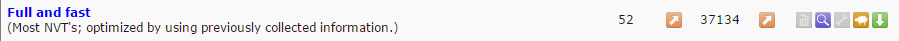
\includegraphics[scale=.4]{figures/full_fast}
  \caption{Vulnerability scan} \label{fig:vulner}
\end{figure}

